\documentclass[10pt, letterpaper]{article}

\usepackage[utf8]{inputenc}
\usepackage[spanish]{babel}
\usepackage{amsmath}
\usepackage{amsfonts}
\usepackage{amssymb}
\usepackage{graphicx}
\usepackage{epstopdf}
\usepackage{url}
\usepackage{booktabs}
\usepackage{caption}
\usepackage{float}
\usepackage{tikz}
\usepackage{subcaption}
\usetikzlibrary{calc}
\usepackage{titlesec}
\usepackage[left=2.2cm, right=2.2cm, top=2.0cm, bottom=2.0cm]{geometry}

\titlespacing*{\section}{0pt}{8pt}{3pt}
\titlespacing*{\subsection}{0pt}{6pt}{2pt}
\setlength{\parskip}{0pt}
\captionsetup{font=small, skip=3pt}

% Estilos del diagrama de bloques
\tikzset{
  bloque/.style={draw, rectangle, align=center, font=\scriptsize,
                 minimum height=0.80cm, inner sep=3pt},
  suma/.style={draw, circle, minimum size=0.58cm, inner sep=0pt,
               font=\footnotesize},
  senal/.style={->, thick, >=latex},
  etiqueta/.style={font=\scriptsize, inner sep=1.5pt}
}


\begin{document}
\begin{center}
    {\LARGE Proyecto --- Parte 1: Especificaciones y modelado cinemático de robot de 2 GdL}
\end{center}
\textbf{Estudiantes: } 
\begin{enumerate}
    \item José Elkin Estrada Morales - \url{estradam_jose@javeriana.edu.co}
    \item Juan David Rodríguez Franco  - \url{juandrodriguezf@javeriana.edu.co}
    \item David Santiago Mojica Lugo -
    \url{david-mojical@javeriana.edu.co}
\end{enumerate}

\section{Métodos y Desarrollos}

\subsection{Introducción y objetivo del proyecto}

El presente proyecto tiene como objetivo diseñar y fabricar un robot manipulador de 2 grados de libertad (GdL) junto a la electrónica necesaria y la implementación de un sistema de control de movimiento. El propósito del robot será trazar una figura de manera autónoma sobre una superficie (como papel; véase la figura \ref{fig:draw_manipu} como referencia). La forma seleccionada por el equipo de trabajo será un triángulo con vértices redondeados (como se muestra en la figura \ref{fig:reul_triag}), conocido matemática y formalmente como ``triángulo de Reuleaux". 

\begin{figure}[H]
    \centering
    % Primera figura (a)
    \begin{subfigure}[b]{0.25\textwidth}
        \centering
        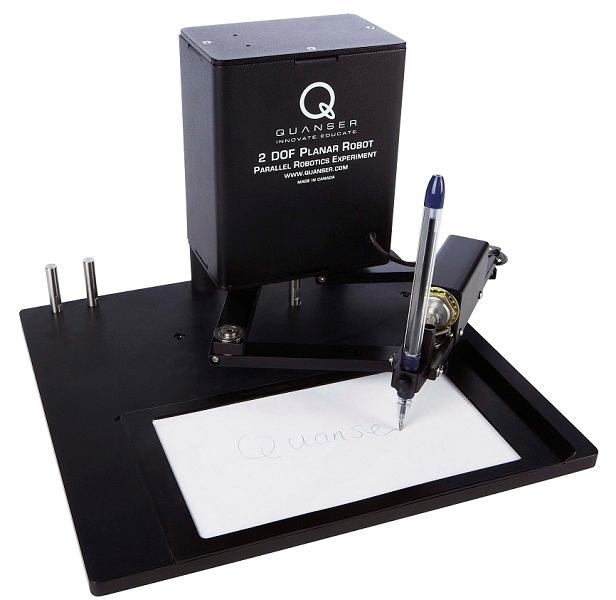
\includegraphics[width=\textwidth]{figuras/quanser.jpg} % Reemplaza por tu primera imagen
        \caption{\textit{Drawing manipulator} de Quanser \cite{barbosa_quanser}.}
        \label{fig:draw_manipu}
    \end{subfigure}
    \hspace{1cm}% Crea un espacio horizontal automático entre ambas figuras
    % Segunda figura (b)
    \begin{subfigure}[b]{0.25\textwidth}
        \centering
        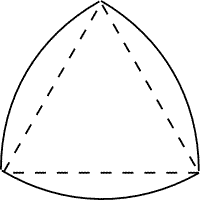
\includegraphics[width=\textwidth]{figuras/triang.png} % Reemplaza por tu segunda imagen
        \caption{Triaángulo de Reuleaux}
        \label{fig:reul_triag}
    \end{subfigure}
    
    % Caption y Label general de todo el conjunto
    \caption{\textbf{Izquierda:} Tipo de robot a diseñar. \textbf{Derecha: }Figura geométrica a realizar.}
    \label{fig:conjunto_figuras}
\end{figure}

La tarea concreta del robot será seguir una trayectoria continua con la geometría del triángulo. Para cumplir con dicho objetivo, el sistema debe, de forma iterativa y por cada punto de la trayectoria mencionada, establecer un modelo de cinemática directa de la posición actual y, justo después, resolver la cinemática inversa de la siguiente \cite{nakamura}, convirtiendo sus coordenadas en el espacio cartesiano en los valores requeridos de las variables articulares para que el efector final alcance dicho punto. La figura \ref{fig:block_diagram} muestra un diagrama de bloques que ilustra el proceso anteriormente mencionado. 

\begin{figure}[H]
    \centering
    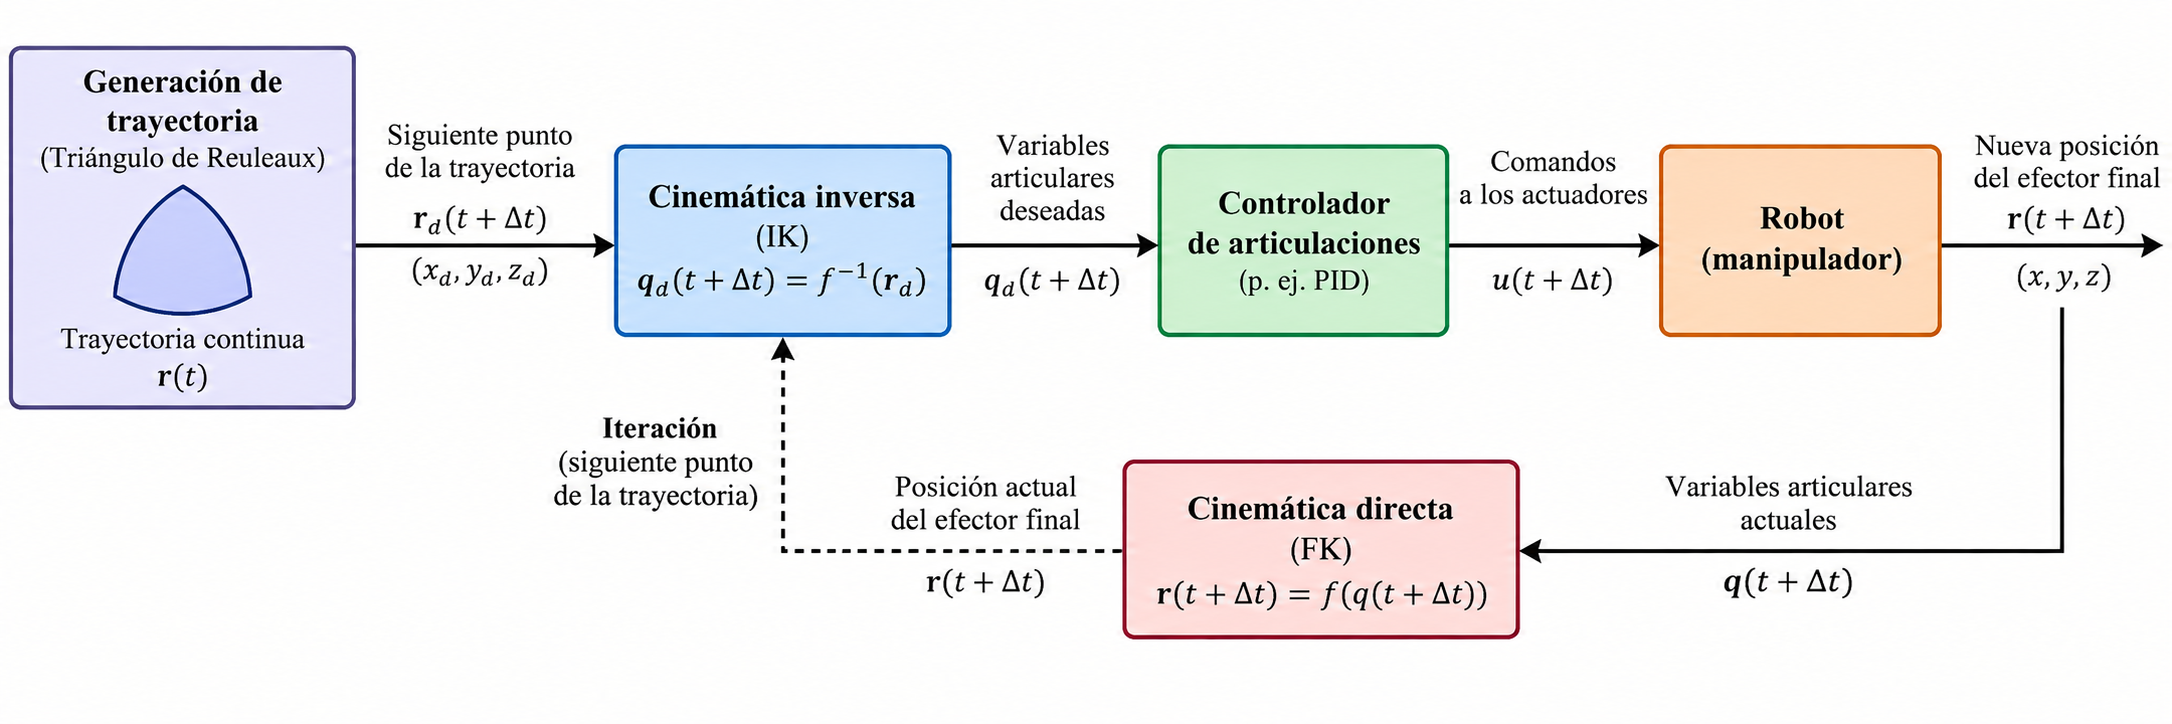
\includegraphics[width=0.75\linewidth]{figuras/block_diagram.png}
    \caption{Diagrama de bloques del funcionamiento del sistema}
    \label{fig:block_diagram}
\end{figure}


\subsection{Requerimientos}

Los requerimientos del robot dependen de aspectos como complejidad de las trayectorias, carga a soportar (en este caso un marcador), el volumen de trabajo y la dexteridad requerida. A continuación se presentan definiciones y más detalles sobre estos aspectos:

\textbf{Complejidad de la trayectoria:} La complejidad de una trayectoria puede cuantificarse a través de las siguientes métricas \cite{spong}: 

\begin{itemize}
    \item \textbf{Continuidad matemática ($C^k$): } En robótica, la continuidad matemática puede entenderse como la propiedad de que los movimientos de un robot no presenten cambios bruscos durante su ejecución \cite{spong}. Por ejemplo, una trayectoria puede clasificarse como $C^0$ si es continua (por ejemplo, que no sea necesario levantar el lápiz del papel para dibujar una figura), como $C^1$ es continua y así sucesivamente. 
    
    \item \textbf{Geometría del perfil y su curvatura: } La curvatura $\kappa$ es una medida de qué tan ``cerrado'' o pronunciado es un cambio de dirección en un punto específico de la trayectoria \cite{spong}. Matemáticamente, puede definirse como $ \kappa = |\dot{x}\ddot{y} - \dot{y}\ddot{x}|/(\dot{x}^2 + \dot{y})^{3/2}$, donde $x(t)$ y $y(t)$ son las coordenadas del marcador en el plano de dibujo a través del tiempo \cite{spong}. 

    \item \textbf{Frecuencia de muestreo y resolución de puntos: } Al seguir una trayectoria, el microcontrolador une cada uno de los puntos moviendo en línea recta el efector final. Si la frecuencia de muestreo es baja o no hay suficientes puntos en la trayectoria, las curvas no estarán bien logradas y la forma final será diferente a la esperada.
\end{itemize}
\textbf{Carga a soportar: } Los marcadores suelen tener una masa aproximadamente de 30 g, lo que implica un peso de 0.294 N. No es una carga significativa.

\textbf{Volumen de trabajo: } Es el conjunto de todos los puntos en el espacio tridimensional o bidimensional $(x, y)$ que el efector final del robot puede alcanzar \cite{spong}. Para un robot de 2 GdL plano, el volumen de trabajo es una región plana 2D con la forma de una semicorona circular con radio interior $R_{min} = L_1 - L_2$ y radio exterior $R_{max} = L_1 + L_2$. Como se verá en la sección \ref{sec:disenio}, se seleccionó $L_1 = 20 \text{ cm}$ y $L_2 = 10 \text{ cm}$. En ese orden de ideas, el volumen de trabajo visualizado desde arriba corresponde a lo ilustrado en la figura \ref{fig:2d_workspace}, mientras que la región 3D por la que el efector final puede desplazarse se muestra en la figura \ref{fig:3d_workspace}.

\begin{figure}[H]
    \centering
    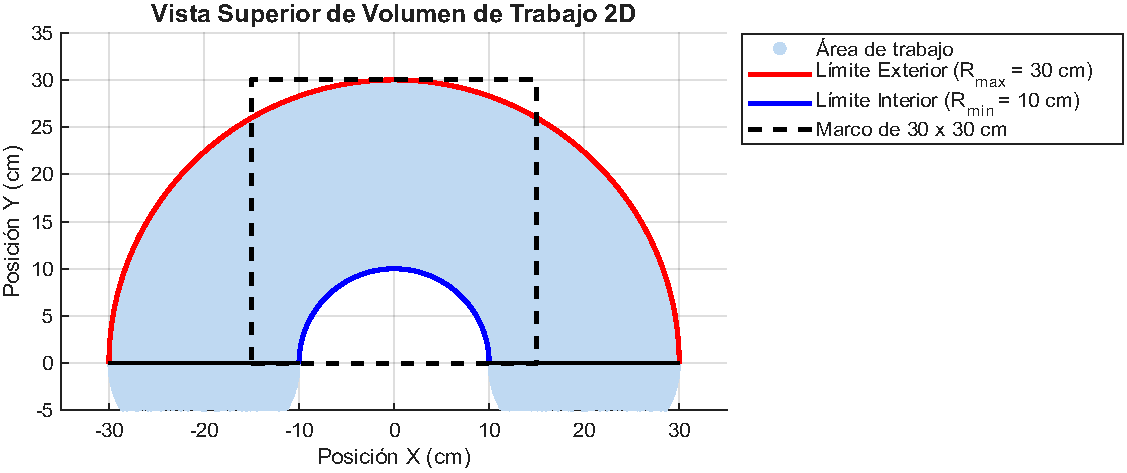
\includegraphics[width=0.6\linewidth]{figuras/2d_workspace.pdf}
    \caption{Volumen de trabajo 2D del robot manipulador}
    \label{fig:2d_workspace}
\end{figure}

\begin{figure}[H]
    \centering
    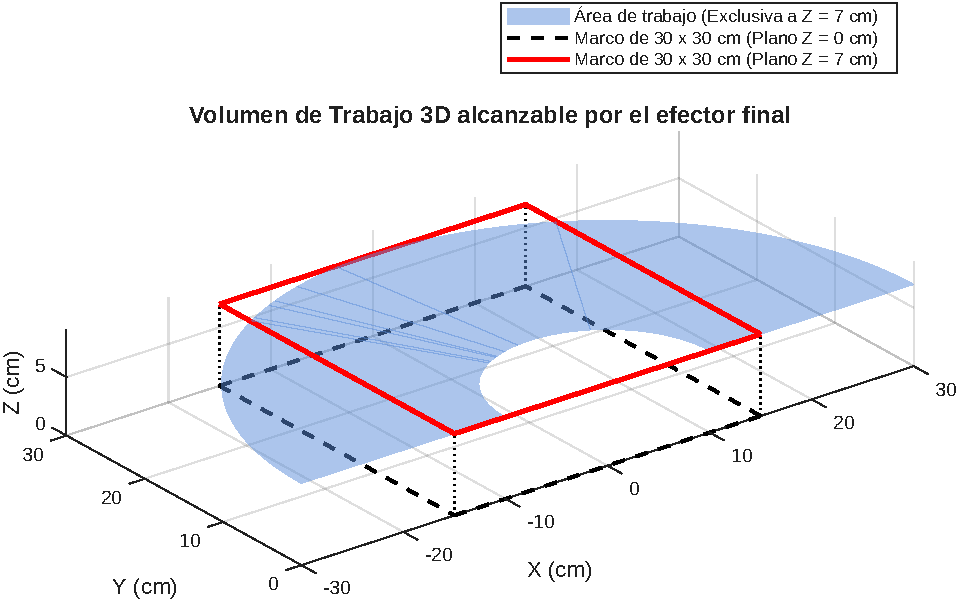
\includegraphics[width=0.6\linewidth]{figuras/3d_workspace.pdf}
    \caption{Volumen de trabajo 3D del robot manipulador}
    \label{fig:3d_workspace}
\end{figure}

\textbf{Dexteridad: } Es la capacidad cinemática del manipulador para cambiar libremente la posición y orientación de de su efector final en un punto específico del espacio de trabajo \cite{spong}. Se cuantifica matemáticamente a partir de la matriz jacobiana $J(q)$ y métricas como el \textbf{Índice de Manipulabilidad de Yoshikawa}, definido como $w(q) = \sqrt{\det(J(q)J^T(q))}$ \cite{spong}. Para robots planares de 2 GdL, $w(q)$ puede escribirse como $w(q) = \vert L_1L_2\sin(\theta_2) \vert$ \cite{spong}, donde $\theta_2$ es el ángulo asociado a la segunda articulación. $w(q)$ mide qué tan ``lejos'' está el robot de una configuración singular. 

Por otra parte, otra métrica es el \textbf{Número de Condición del Jacobiano} \cite{spong}, expresado como
 
\begin{equation*}
   \kappa(J) = \Vert J \Vert \cdot \Vert J^{-1} \Vert = \frac{\sigma_{max}}{\sigma_{min}},
\end{equation*}

donde $\sigma_{max}$ y $\sigma_{min}$ son, respectivamente, los valores singulares máximos y mínimos de $J$. 

Teniendo en cuenta todos los aspectos mencionados anteriormente, los requerimientos establecidos para el sistema se muestran en la tabla \ref{tab:requerimientos}.

\begin{table}[H]
    \centering
    \caption{Requerimientos del sistema}
    \label{tab:requerimientos}
    \begin{tabular}{|p{4.5cm}|p{4.5cm}|p{6cm}|}
    \hline
    \textbf{Especificación} & \textbf{Métrica} & \textbf{Breve justificación} \\ \hline
    Continuidad matemática & $C^1$ (posición y velocidad continuas) & Garantiza transiciones suaves de movimiento \\ \hline
    Velocidad cartesiana en los vértices & $v \to 0$ (tendiendo a cero) & Prevenir discontinuides en la función de curvatura $\kappa$. \\ \hline
    Tiempo de muestreo & $\Delta t \le 0.01$ s ($f_s \ge 100$ Hz) & Garantizar un seguimiento fino y evitar la poligonalización del trazado curvo. \\ \hline
    Orden polinómico de interpolación & Polinomios de orden 3 (splines cúbicos) & Asegura la continuidad $C^1$, proporcionando perfiles de velocidad continuos. \\ \hline
    Capacidad de carga útil (Payload) & $\ge 0.294$ N ($30$ g) & Garantizar el soporte del marcador sin afectar la dinámica. \\ \hline
    Alcance radial de la zona de trabajo & Semicorona circular con $R_{min} = 10$ cm y $R_{max} = 30$ cm & Contener al triángulo de Reuleaux, alejándolo de los límites físicos y configuraciones singulares del brazo. \\ \hline
    Límite del Índice de Yoshikawa & Evitar $\theta_2 = 0^\circ$ y $\theta_2 = 180^\circ$ & Evitar la pérdida de grados de libertad por efecto de singularidades. \\ \hline
    Número de Condición del Jacobiano & $\kappa(J)$ cercano a $1$ ($\kappa(J) \ll \infty$) & Evitar configuraciones singulares (de forma parecida al índice de Yoshikawa) \\ \hline
    \end{tabular}
\end{table}
 
\subsection{Componentes}

Los componentes necesarios para el robot se muestran en la tabla \ref{tab:compos}.

\begin{table}[H]
    \centering
    \caption{Componentes del sistema con características, función y costos asociados}
    \label{tab:compos}
    \begin{minipage}{15.2cm} % Ajustado a la suma de las columnas: 3.2 + 4.5 + 4.5 + 2.2 = 14.4cm + márgenes
        \centering
        \begin{tabular}{|p{3.2cm}|p{4.5cm}|p{4.5cm}|p{2.2cm}|}
        \hline
        \textbf{Componente} & \textbf{Características} & \textbf{Función} & \textbf{Costo (COP)} \\ \hline
        Servomotores Futaba S3003 (x2) & \textbf{Torque:} 4.1 kg-cm \newline \textbf{Voltaje:} 6 V \newline \textbf{Rotación:} 180$^\circ$ \newline \textbf{Velocidad*:} 0.19 s / 60$^\circ$ & Actuadores & \$37 800 \\ \hline
        Microcontrolador ESP32-S3 & Procesador Xtensa® LX7 de doble núcleo \newline 16 MB de memoria Flash \newline 8 MB de memoria PSRAM & Solución de problemas cinemáticos, control de movimiento e interpolación de trayectorias. & Posesión del equipo \\ \hline
        Lámina de balso & Tamaño & Material para base y eslabones. & \$20 000 \\ \hline
        Marcador Sharpie & Color negro & Dibujo & \$2 500 \\ \hline
        \end{tabular}
        
        \vspace{1.5mm} % Controla la cercanía del texto con la tabla
        \raggedright \footnotesize $^*$ Como puede intuirse, las velocidades máximas articulares del robot coinciden con las velocidad de los servomotores.
    \end{minipage}
\end{table}

\subsection{Diseño y modelo CAD}
\label{sec:disenio}

\subsection{Modelo cinemático directo (Denavit-Hartenberg)}
\label{sec:dh}

El robot es un manipulador plano de 2 grados de libertad (2R): ambas
articulaciones son rotacionales ($\sigma_i = 0$) con ejes $z$ paralelos y
perpendiculares al plano de dibujo. La tabla \ref{tab:dh} resume los parámetros
de Denavit-Hartenberg en la convención estándar; las longitudes $L_1 = 0.200$ m
y $L_2 = 0.100$ m se tomaron del modelo CAD (de centro de eje a centro de eje).

\begin{table}[H]
    \centering
    \caption{Parámetros Denavit-Hartenberg del robot (convención estándar).}
    \label{tab:dh}
    \begin{tabular}{cccccc}
    \toprule
    Eslabón & $\theta_i^{off}$ [rad] & $d_i$ [m] & $a_i$ [m] & $\alpha_i$ [rad] & $\sigma_i$ \\
    \midrule
    1 & 0 & $d_1 = 0$     & $L_1 = 0.200$ & 0 & 0 \\
    2 & 0 & 0             & $L_2 = 0.100$ & 0 & 0 \\
    \bottomrule
    \end{tabular}
\end{table}

La transformación homogénea que relaciona los marcos $i-1$ e $i$ es

\begin{equation}
{}^{i-1}_{i}T =
\begin{bmatrix}
\cos\theta_i & -\sin\theta_i\cos\alpha_i & \sin\theta_i\sin\alpha_i & a_i\cos\theta_i \\
\sin\theta_i &  \cos\theta_i\cos\alpha_i & -\cos\theta_i\sin\alpha_i & a_i\sin\theta_i \\
0            &  \sin\alpha_i              &  \cos\alpha_i            & d_i \\
0            &  0                         &  0                       & 1
\end{bmatrix},
\label{eq:dh_mat}
\end{equation}

con $\theta_i = q_i + \theta_i^{off}$. Como $\alpha_1 = \alpha_2 = 0$, las
transformaciones individuales resultan

\begin{equation}
{}^{0}_{1}T =
\begin{bmatrix}
c_1 & -s_1 & 0 & L_1 c_1 \\
s_1 &  c_1 & 0 & L_1 s_1 \\
0   &  0   & 1 & d_1 \\
0   &  0   & 0 & 1
\end{bmatrix},
\qquad
{}^{1}_{2}T =
\begin{bmatrix}
c_2 & -s_2 & 0 & L_2 c_2 \\
s_2 &  c_2 & 0 & L_2 s_2 \\
0   &  0   & 1 & 0 \\
0   &  0   & 0 & 1
\end{bmatrix},
\label{eq:A1A2}
\end{equation}

donde $c_i = \cos q_i$ y $s_i = \sin q_i$. El producto acumulativo
${}^{0}_{2}T = {}^{0}_{1}T\,{}^{1}_{2}T$ da la posición del efector final,

\begin{equation}
\begin{bmatrix} x \\ y \\ z \end{bmatrix} =
\begin{bmatrix}
L_1\cos q_1 + L_2\cos(q_1 + q_2) \\
L_1\sin q_1 + L_2\sin(q_1 + q_2) \\
d_1
\end{bmatrix},
\label{eq:fk}
\end{equation}

y una orientación que es una rotación $\phi = q_1 + q_2$ sobre el eje $z$. La
función \texttt{forward\_kinematics(DH,q)} implementa la ecuación
\eqref{eq:dh_mat} de forma genérica para $n$ eslabones: parte de $T = I_4$ y
acumula $T \leftarrow T \cdot {}^{i-1}_{i}T$ para $i = 1, \dots, n$. Admite un
vector $q$ o una matriz $N \times n$ (trayectoria), en cuyo caso retorna un
arreglo $4 \times 4 \times N$.

\section{Resultados}

\subsection{Cinemática directa}

La cinemática directa se evaluó en $q = [60^\circ, -50^\circ]$ y se comparó con
la solución analítica (\eqref{eq:fk}) y con \texttt{SerialLink.fkine} del
Robotics Toolbox. La tabla \ref{tab:fk_val} resume el resultado: la posición
calculada coincide con la analítica y con el toolbox con un error máximo de
$2.8\times10^{-17}$ m. Además, el producto numérico de las matrices
${}^{0}_{1}T\,{}^{1}_{2}T$ coincide exactamente con
\texttt{forward\_kinematics}, lo que valida la implementación.

\begin{table}[H]
    \centering
    \caption{Validación de la cinemática directa en $q = [60^\circ, -50^\circ]$.}
    \label{tab:fk_val}
    \begin{tabular}{lccc}
    \toprule
    Método & $x$ [m] & $y$ [m] & $z$ [m] \\
    \midrule
    Implementación propia & 0.19848078 & 0.19056990 & 0 \\
    Solución analítica    & 0.19848078 & 0.19056990 & 0 \\
    \texttt{SerialLink.fkine()} & 0.19848078 & 0.19056990 & 0 \\
    \bottomrule
    \end{tabular}
\end{table}

La figura \ref{fig:cin_dir} muestra el esquema del brazo en esa configuración,
con los marcos de Denavit-Hartenberg y el volumen de trabajo: una corona con
$R_{min} = L_1 - L_2 = 0.1$ m y $R_{max} = L_1 + L_2 = 0.3$ m que contiene al
triángulo de Reuleaux (en azul).

\begin{figure}[H]
    \centering
    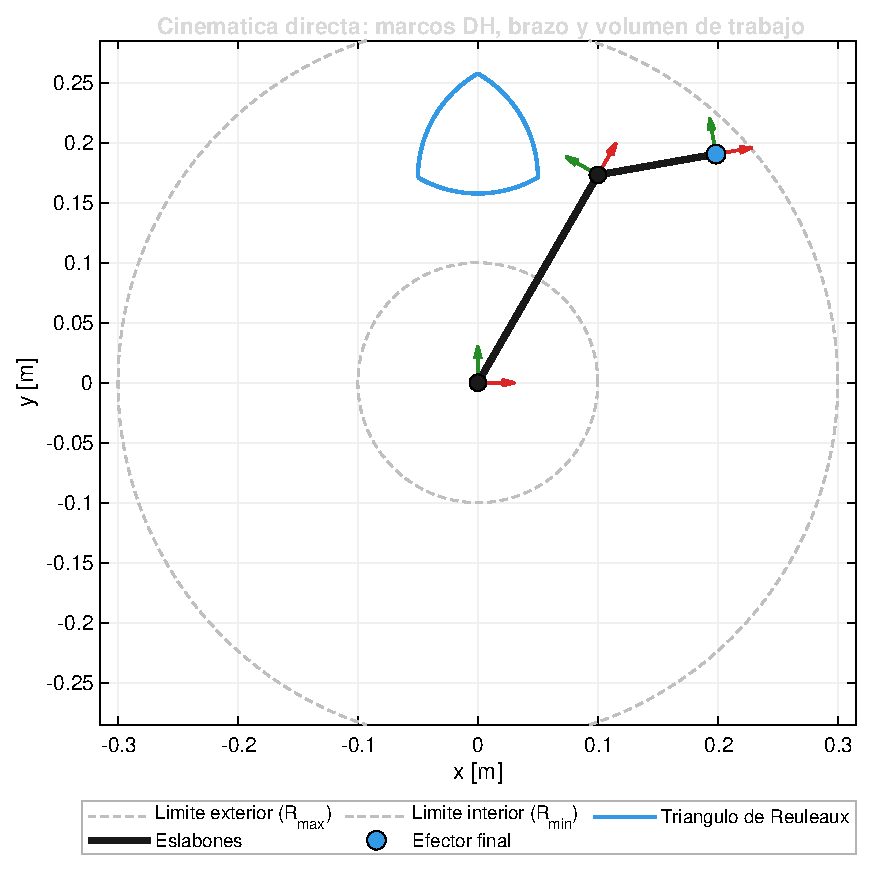
\includegraphics[width=0.68\textwidth]{figuras/cinematica_directa_esquema.eps}
    \caption{Cinemática directa: marcos DH, brazo en $q = [60^\circ, -50^\circ]$
    y volumen de trabajo.}
    \label{fig:cin_dir}
\end{figure}

\subsection{Cinemática inversa}

\subsection{Planeación de trayectorias}


\section{Conclusiones}


\bibliographystyle{ieeetr} % Define el estilo de formato (puedes cambiarlo por plain, unsrt, etc.)
\bibliography{referencias} % Llama a tu archivo .bib (no incluyas la extensión .bib aquí)


\end{document}